\documentclass{article}

%%%%%%%%%%%%%%%%%%%%%%%%%%%%%%%%%%%%%%%%%%%%%%%%%%%%%%%%%%%%%%%%%
%package

%geometry
\usepackage[a4paper]{geometry}%调整页面边距
\geometry{left=3cm,right=3cm,top=3cm,bottom=3cm}
\linespread{1.5}
\usepackage{fancyhdr}%梦幻页眉

%fonts
\usepackage{fontspec}%字体库
\defaultfontfeatures{Mapping=tex-text}
\usepackage{xunicode,xltxtra}
\usepackage[BoldFont,SlantFont,CJKnumber,CJKchecksingle]{xeCJK}  % \CJKnumber{12345}: 一万二千三百四十五
\usepackage{CJKfntef}
\usepackage{bm} %公式中的粗体字符\boldsymbol
\usepackage{pifont}

%color
\usepackage{color,xcolor}
\definecolor{GREEN}{RGB}{25,180,68}
\definecolor{YELLOW}{RGB}{255,255,224}
\definecolor{BLUE}{RGB}{9,148,234}
\definecolor{RED}{RGB}{139,0,0}
\definecolor{DRED}{RGB}{128,0,0}
\definecolor{GREY}{RGB}{128,128,128}
\usepackage[pagecolor={YELLOW}]{pagecolor}%设置页面底色

%math
\usepackage{amsmath,amsfonts,amssymb}

%graphics
\usepackage[americaninductors,europeanresistors]{circuitikz}
\usepackage{tikz}%可以绘制各种坐标图,方格图
\usetikzlibrary{positioning,arrows,shadows,shapes,calc,mindmap,trees,backgrounds}  % placements=positioning
\usepackage{graphicx}%\includegraphics插图命令
\usepackage{subfigure}  %%图形或表格并排排列

% table
\usepackage{colortbl,dcolumn}  %% 彩色表格
\usepackage{multirow}
\usepackage{multicol}
\usepackage{booktabs}

% code
\usepackage{fancyvrb}%漂亮的代码包
\usepackage{listings}%加入代码

% ref
\usepackage{hyperref}%扩展参考文献,目录功能和加入超链接。

% title
\usepackage{titlesec}%花哨的章节标题

\usepackage{etoolbox}
\makeatletter
\patchcmd{\ttlh@hang}{\parindent\z@}{\parindent\z@\leavevmode}{}{}
\patchcmd{\ttlh@hang}{\noindent}{}{}{}
\makeatother%titlesec旧版本无编号问题


\titleformat
{\section} % command
[display] % shape
{\bfseries\Large} % format
{第\ \thesection 章\ } % label
{0.3ex} % sep
{
    \rule{\textwidth}{1pt}
    \vspace{1ex}
    \centering
} % before-code
[
\vspace{-2ex}%
\rule{\textwidth}{1pt}
] % after-code


%tightly-packed lists
\usepackage{mdwlist}
\usepackage{verbatim}%comment命令的注释包
\usepackage{styles/zhfontcfg}%中文包
\usepackage{styles/visionouclistings}
\usepackage{styles/visionouccfg}

% head/foot
\setlength{\headheight}{15pt}

\fancyhf{}



%%%%%%%%%%%%%%%%%%%%%%%%%%%%%%%%%%%%%%%%%%%%%%%%%%%%%%%%%%%%%%%%%%%%%%

%settings
\setCJKmainfont{Adobe Kaiti Std} %设置为楷体
\setCJKmonofont{Adobe Fangsong Std}%仿宋
%页眉页脚


\makeatletter
\def\headrule{{\if@fancyplain\let\headrulewidth\plainheadrulewidth\fi%
\hrule\@height 2.5pt \@width\headwidth\vskip1pt%上面线为2.5pt粗  
\hrule\@height 0.5pt\@width\headwidth  %下面0.5pt粗            
\vskip-2\headrulewidth\vskip-1pt}      %两条线的距离        
\vspace{6mm}}     %双线与下面正文之间的垂直间距              
\makeatother         
 

% graphics
\graphicspath{{figures/}}
\tikzset{
    % Define standard arrow tip
    >=stealth',
    % Define style for boxes
    punkt/.style={
           rectangle,
           rounded corners,
           draw=black, very thick,
           text width=6.5em,
           minimum height=2em,
           text centered},
    % Define arrow style
    pil/.style={
           ->,
           thick,
           shorten <=2pt,
           shorten >=2pt,},
    % Define style for FlyZhyBall
    FlyZhyBall/.style={
      circle,
      minimum size=6mm,
      inner sep=0.5pt,
      ball color=red!50!blue,
      text=white,},
    % Define style for FlyZhyRectangle
    FlyZhyRectangle/.style={
      rectangle,
      rounded corners,
      minimum size=6mm,
      ball color=red!50!blue,
      text=white,},
    % Define style for zhyfly
    zhyfly/.style={
      rectangle,
      rounded corners,
      minimum size=6mm,
      ball color=red!25!blue,
      text=white,},
    % Define style for new rectangle
    nrectangle/.style={
      rectangle,
      draw=#1!50,
      fill=#1!20,
      minimum size=5mm,
      inner sep=0.1pt,}
}

% code
\lstnewenvironment{VHDLcode}[1][]{%
  \lstset{
    basicstyle=\footnotesize\ttfamily\color{black},%
    columns=flexible,%
    framexleftmargin=.7mm,frame=shadowbox,%
    rulesepcolor=\color{blue},%
%    frame=single,%
    backgroundcolor=\color{yellow!20},%
    xleftmargin=1.2\fboxsep,%
    xrightmargin=.7\fboxsep,%
    numberstyle=\tiny\color{blue},%
    numberblanklines=false,numbersep=7pt,%
    language=VHDL%
    }\lstset{#1}}{}
\lstnewenvironment{VHDLmiddle}[1][]{%
  \lstset{
    basicstyle=\scriptsize\ttfamily\color{black},%
    columns=flexible,%
    framexleftmargin=.7mm,frame=shadowbox,%
    rulesepcolor=\color{blue},%
%    frame=single,%
    backgroundcolor=\color{yellow!20},%
    xleftmargin=1.2\fboxsep,%
    xrightmargin=.7\fboxsep,%
    numbers=left,numberstyle=\tiny\color{blue},%
    numberblanklines=false,numbersep=7pt,%
    language=VHDL%
    }\lstset{#1}}{}
\lstnewenvironment{VHDLsmall}[1][]{%
  \lstset{
    basicstyle=\tiny\ttfamily\color{black},%
    columns=flexible,%
    framexleftmargin=.7mm,frame=shadowbox,%
    rulesepcolor=\color{blue},%
%    frame=single,%
    backgroundcolor=\color{yellow!20},%
    xleftmargin=1.2\fboxsep,%
    xrightmargin=.7\fboxsep,%
    numbers=left,numberstyle=\tiny\color{blue},%
    numberblanklines=false,numbersep=7pt,%
    language=VHDL%
    }\lstset{#1}}{}
% pdf
\hypersetup{pdfauthor={Haiyong Zheng},%
            pdftitle={Title},%
            CJKbookmarks=true,%
            bookmarksnumbered=true,%
            bookmarksopen=false,%
            plainpages=false,%
            colorlinks=true,%
            citecolor=green,%
            filecolor=magenta,%
            linkcolor=DRED,%red(default)
            urlcolor=cyan}
\newcommand\titlebar{%
\tikz[baseline,trim left=3.1cm,trim right=3cm] {
    \fill [cyan!25] (2.5cm,-1ex) rectangle (\textwidth+3.1cm,2.5ex);
    \node [
        fill=cyan!60!white,
        anchor= base east,
        rounded rectangle,
        minimum height=3.5ex] at (3cm,0) {
        \textbf{\thesection.}
    };
}%
}

%设置标题页面

% newcommand*{\titleGM}{\begingroup % 新命令:添加标题页
%\hbox{ % 水平盒子
%\hspace*{0.2\textwidth} % 左边空白
%\rule{1pt}{\textheight\color{GREY}} % 竖线
%\hspace*{0.05\textwidth} % 竖线和文本距离
%\parbox[b]{0.75\textwidth}{ % 文本最大右边距

%{\noindent\Huge\bfseries \LaTeX \\[0.5\baselineskip] - Getting Started}\\[2\baselineskip] % 题目
%{\large \textit{一份\LaTeX 入门手册}}\\[4\baselineskip] % 标签或描述
%{\Large \textsc{丁昊}}\\ % 作者

%\vspace{0.5\textheight} % 题目区域和作者间距
%{\noindent Augest 2016 }\\[\baselineskip] % Publisher and logo
%}}
%\endgroup}


\usepackage{styles/lshort}

%%%%%%%%%%%%%%%%%%%%%%%%%%%%%%%%%%%%%%%%%%%%%%%%%%%%%%%%%%%%%%%%%
\begin{document}
\title{\vspace{-2em}Ubuntu 16.04安装教程及入门\vspace{0.7em}}%大标题
\author{谭琳}%作者
\date{\vspace{-0.7em}2016年8月\vspace{-0.7em}}%日期
\maketitle\thispagestyle{fancy}%在上部添加横线

\pagenumbering{roman}

\setcounter{page}{0}
%\newpage

%\begin{abstract}
%这篇文档作者写的虽然是我的名字,事实上却是因为我很难把那么多名字统统写进来。首先,本文档后半部分内容主要来源于孙雪,戴嘉伦两位师兄师姐和郑海永老师的《\LaTeX 简短使用手册》。版式的设置部分参照了常琳师姐的文档模板,并采取了崔金娜、谭琳和王超的很多建议。写这篇文档的过程对我也是个挑战,郑老师帮我解决了一系列编写中遇到的问题。且本文的绝大部分实际内容来自于官方编写的《一份不太简短的\LaTeXe 介绍》(后文简称为《介绍》),所以说我实际上是做了大量整理工作而非原创性工作。\par
%但是到目前为止,上面提到的这些及网上的文档要不太长,要不难以满足翻遍电脑找不到\LaTeX 可执行文件在哪的初学级菜鸟的需求,我尽我最大的努力给予一些我在那个阶段最想要知道的一些信息,尽量的总结至一天可以学会的量,而不再需要你们将一整天又一整天的时间耗费在百度和谷歌上。\par
%最后,我个人的水平着实有限,希望这份文档可以被不断的修改和更新,并以更好的样子服务更多的师弟师妹。
%\end{abstract}

\newpage

\tableofcontents 
\newpage

\pagestyle{fancy}

\pagenumbering{arabic}
\newpage
 \chead{\color{GREY}Ubuntu 16.04 Installation Tutorial And Menu}%页眉
\cfoot{\color{GREY}Augeust 2016}%页脚 中
\lfoot{\color{GREY}TanLin}%页脚 左
\rfoot{\color{GREY}$\cdot$\ Page \thepage\ }%页脚 右
\renewcommand{\headrulewidth}{0.4pt}
\renewcommand{\footrulewidth}{0.4pt}
            

\section{Ubuntu的安装}

现在实验室用的是Ubuntu16.04,至于版本根据Ubuntu官方出的最新版为准,因为Ubuntu的安装近乎相同,这里以Ubuntu16.04的安装为例进行说明。

\subsection{Ubuntu的下载}

  在Ubuntu官网上下载\url{http://cn.ubuntu.com/download/},如果你电脑的内存少于2GB,选择32位下载,我选择下载的的是64位。下载下来是一个ubuntu-16.04-desktop-amd64.iso的镜像文件,这个下载过程有点长,需要你耐心等待哦!

\subsection{U盘启动器的制作}
\begin{enumerate}
\item 在安装Ubuntu之前需要做一个硬件启动器,你可以用easyBCD软件来安装,也可以用U盘来制作U盘启动器,二者我都用过,觉得还是U盘比较简单,这里我就以制作U盘为例。

\item 首先找个最好是8G的空U盘,插在你的电脑上备用。然后在百度上可以搜软碟通ultraiso,这个在Windows7和Windows8都可以下载。下载完成后打开ultraiso,点击工具栏的“打开”按钮,选择第一步下载的ubuntu-16.04-desktop-amd64.iso打开。

\item 再点击工具栏里的“启动”,在弹出的框里,点击“写入硬盘映像”,如图\ref{tu1}所示。
\begin{figure}[!htb] %插图
\centering
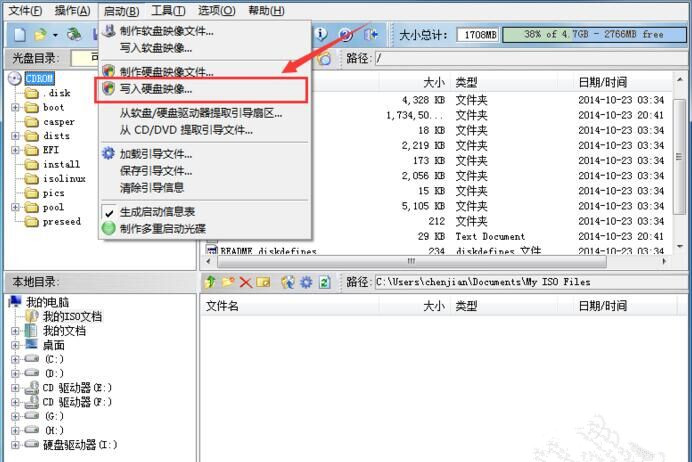
\includegraphics[width=0.6\textwidth]{tu1.jpeg}
\caption{\small 写入硬盘映像}
\label{tu1}
\end{figure}  

\item 此时,在弹出的框内,硬盘驱动器是你的U盘名,写入方式是USB-DD。下面一步是我们制作的U盘启动器能否启动电脑的关键,点击“便捷启动”,选择“写入新的驱动器引导扇面去”的“Syslinux”。随后,会弹出很多提示框,你可以一路点是到底,这一步的Syslinux写入很快的,最后会提示你安装成功,如若不然,你可重复上面的步骤。如图\ref{tu2}图\ref{tu3}所示。
\begin{figure}[!htb] %插图
\centering
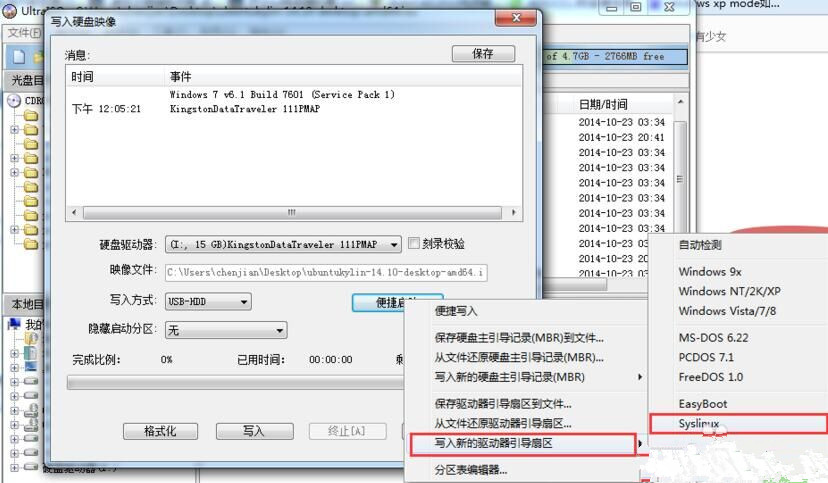
\includegraphics[width=0.6\textwidth]{tu2.jpeg}
\caption{\small 写入Syslinux}
\label{tu2}
\end{figure}  

\begin{figure}[!htb] %插图
\centering
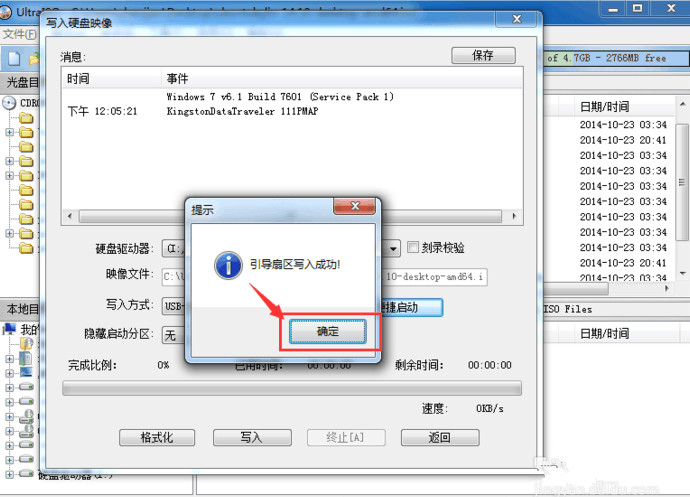
\includegraphics[width=0.6\textwidth]{tu3.jpeg}
\caption{\small Syslinux写入成功}
\label{tu3}
\end{figure}  
\item 制作U盘启动器的最后一步就是,点击“写入”,大约此过程需要等待写入完成5分钟,随后,在消息里可以看到“刻录成功”,我们点击“返回”即可,如图\ref{tu5}所示。
\begin{figure}[!htb] %插图
\centering
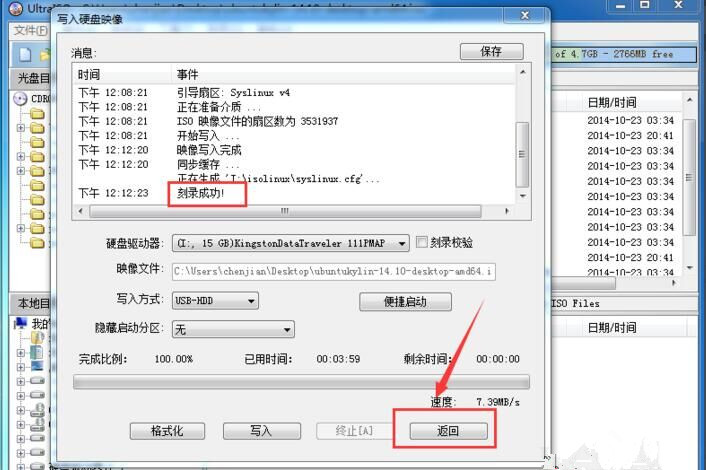
\includegraphics[width=0.6\textwidth]{tu5.jpeg}
\caption{\small 刻录成功}
\label{tu5}
\end{figure}\\ 
\textsl{此时,我们的U盘启动器就制作好了,我们可以安装我们的Ubuntu啦!}
\end{enumerate}
\subsection{Ubuntu的安装}

\subsubsection{Ubuntu单系统安装}
\begin{enumerate}

\item  刚刚安装好的U盘启动器不用拔出,直接重启电脑,一直按快捷键进入boot界面。各款电脑常用快捷键有:笔记本 联想、宏基、三星、方正、海尔、清华同方、戴尔、神舟 F12,华硕、索尼 ESC,惠普、明基 F9;台式机 联想、惠普、宏基、神舟、方正、海尔、清华同方 F12,戴尔 ESC,华硕、明基 F8。

\item  进入boot界面后,选择“USB”那个栏安装,如下图\ref{tu6}所示(因为我按的就是Ubuntu,所以有好几个USB选项,第一次装的话,那么就一个)。

\begin{figure}[!htb] %插图
\centering
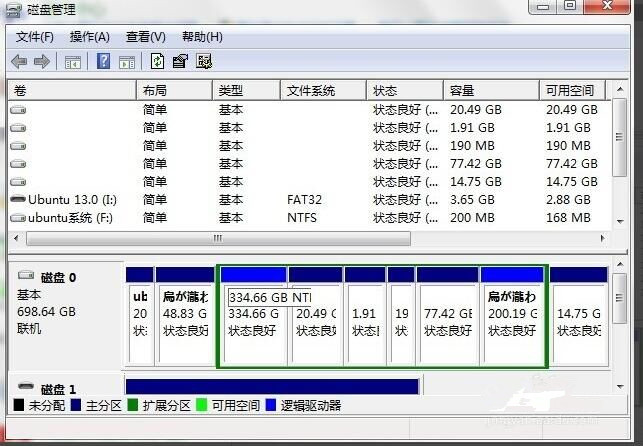
\includegraphics[width=0.5\textwidth]{tu6.jpeg}
\caption{\small USB选择}
\label{tu6}
\end{figure} 

\item  进入之后,在左侧选择“中文(简体)”,那么右侧就出现了如下图\ref{tu7}所示的安装界面,点击“安装Ubuntu”。

\begin{figure}[!htb] %插图
\centering
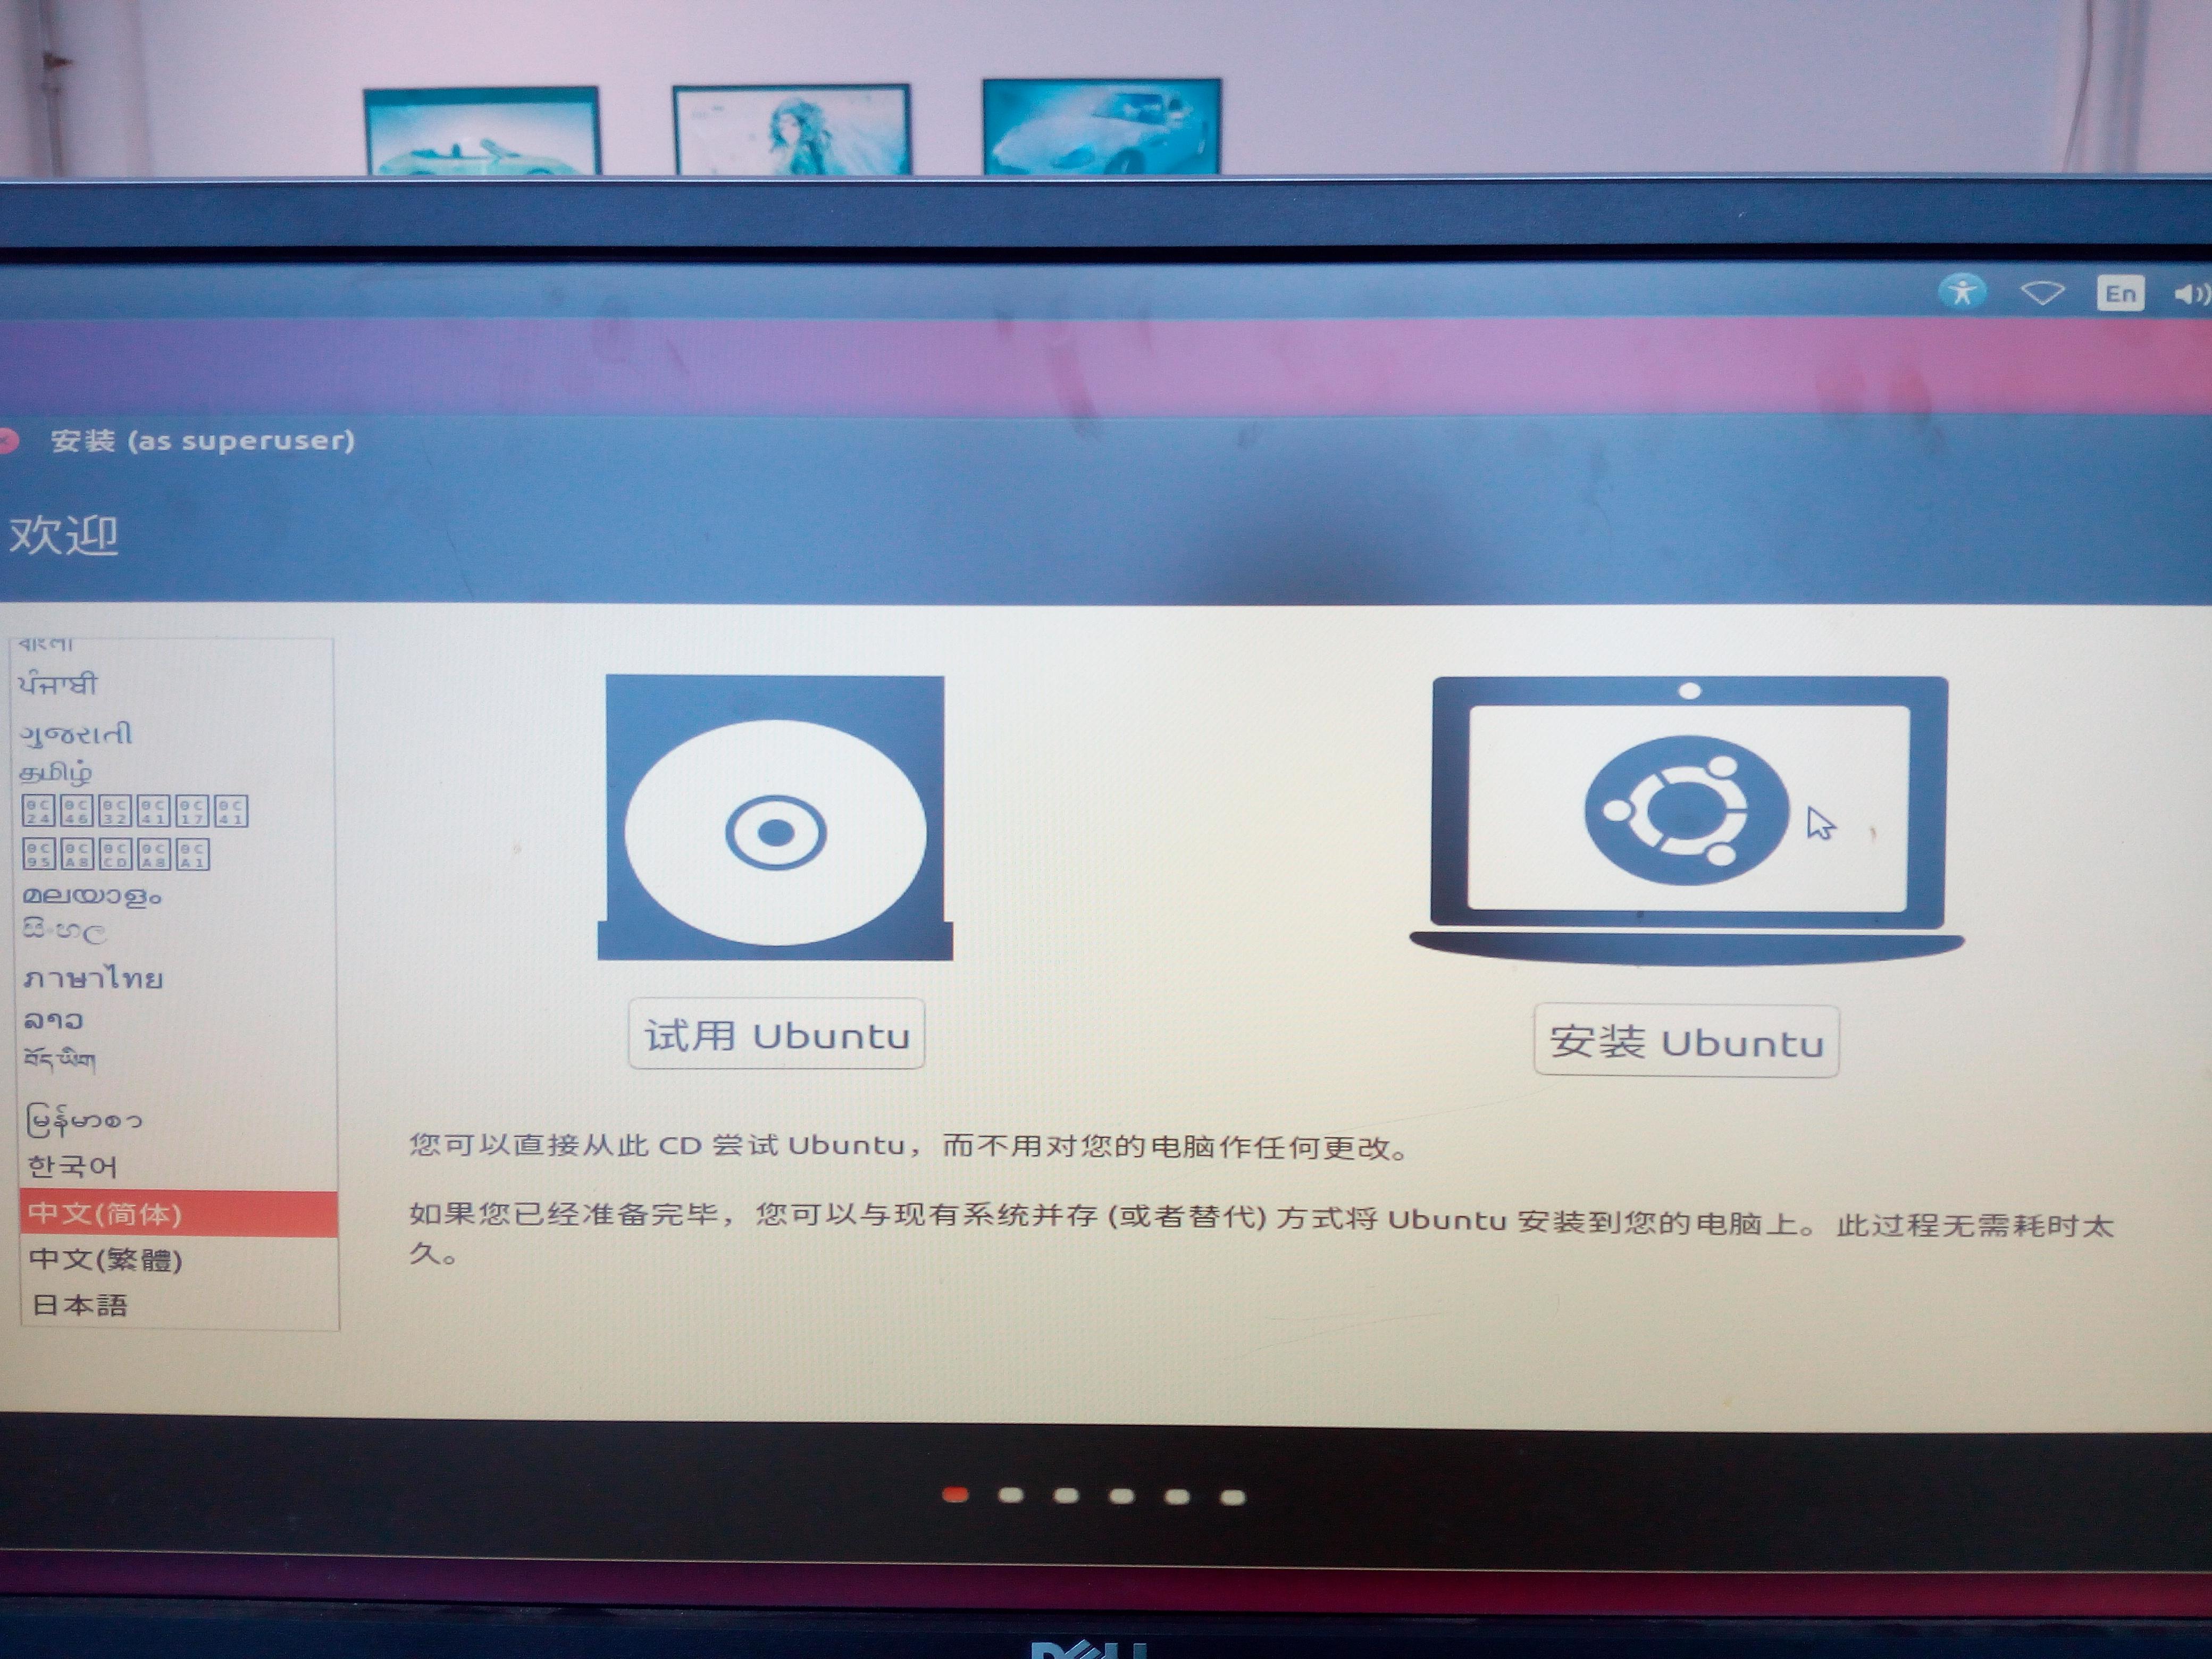
\includegraphics[width=0.5\textwidth]{tu7.jpeg}
\caption{\small 安装Ubuntu}
\label{tu7}
\end{figure}
 
\item   在出现的提示框下\ref{tu8},一般是不选择,直接按“继续”。

\begin{figure}[!htb] %插图
\centering
\includegraphics[width=0.5\textwidth]{tu8.jpeg}
\caption{\small 准备安装}
\label{tu8}
\end{figure} 

\item  随后出现安装类型,如下图\ref{tu9},(因为我已经安装了Ubuntu16.04),如果你原先是Windows7,你想保留Windows7的一些文档、音乐、其他文件可以选择第二个与你原先的并存。在实验室,一般都是单系统,所以你也以选择第三项清除整个磁盘,但是这样在运行一些程序有点卡。所以一般还是选择按“其他选项”,这样可以自己分区,如果你想安装双系统的话,一定的选{\color{red}“其他选项”},至于安装双系统教程下面会说。点击“继续”。

\begin{figure}[!htb] %插图
\centering
\includegraphics[width=0.5\textwidth]{tu9.jpeg}
\caption{\small ubuntu安装类型}
\label{tu9}
\end{figure} 
\begin{figure}[!htb] %插图
\centering
\includegraphics[width=0.5\textwidth]{tu10.jpeg}
\caption{\small Ubuntu分区}
\label{tu10}
\end{figure} 

\item  进入分区界面\ref{tu10}。单击左下角“-”是删除分区,“+”是创建分区。Ubuntu分区一般有$\slash$boot、$\slash$swap、$\slash$、$\slash$home、$\slash$op 五个挂载点。实验室一般安装的都是单系统,这里以安装单系统内存为8G,硬盘空间500G为例,说一下分区。

分区类型选的 都是“逻辑分区”,新分区的位置选择,是“空间起始位置”。

\begin{verbatim}
/boot,单系统不用分

/    ,分大约65G就行 ,用于Ext4日志文件系统

/home,分大约250G就行,用于Ext4日志文件系统

/swap,内存在4G以上可以不用考虑,如果要分的话,分大约是内存的1.5-2倍,用于交换空间

/opt ,余下的都分在这个区,用于用于Ext4日志文件系统
\end{verbatim}

\item   分区分好之后选择“现在安装”。

\item 出现您在什么地方的提示框,你只要单击“继续”就可以了。图\ref{tu12}所示

\begin{figure}[!htb] %插图
\centering
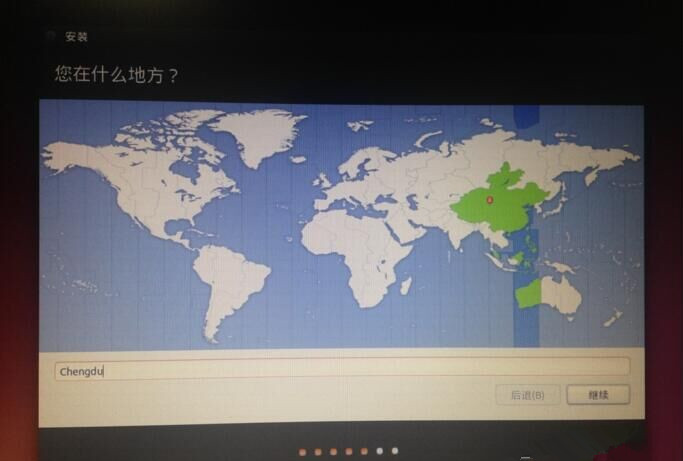
\includegraphics[width=0.4\textwidth]{tu12.jpeg}
\caption{\small 地点提示}
\label{tu12}
\end{figure} 

\item  在键盘布局选择英语(美国),点击“继续”。图\ref{tu13}所示
\begin{figure}[!htb] %插图
\centering
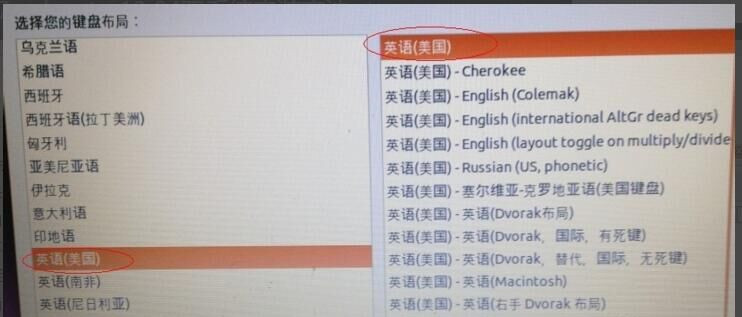
\includegraphics[width=0.4\textwidth]{tu13.jpeg}
\caption{\small 键盘布局选择}
\label{tu13}
\end{figure} 

\item  填写个人信息,名字密码,单击“继续”。

\item  进入到了安装界面,等待安装。

\begin{figure}[!htb] %插图
\centering

\includegraphics[width=0.5\textwidth]{tu14.jpeg}
\caption{\small 重启提示}
\label{tu14}
\end{figure} 
\end{enumerate}
安装完成后,你需要的是重启电脑,图\ref{tu14}所示。开机画面是这样的,你需要输入刚才设置的密码即可。此时你的Ubuntu就安装上了你可以使用了哦!

\subsubsection{Ubuntu双系统安装}

如果你要装双系统的话,\textsl{{\color{red}温馨提示一下},{\color{blue}如果新手的话,操作难免会失误,因此,建议大家操作前,切记注意备份重要数据,本人就是一个血淋淋的例子}。}
\begin{enumerate}
\item 双系统也需要下载,制作u盘启动器,在安装之前需要在分区这里用Windows7自带的磁盘管理进行分区,打开方法:右键计算机-管理-磁盘管理。如图\ref{tu21}所示
\begin{figure}[!htb] %插图
\centering
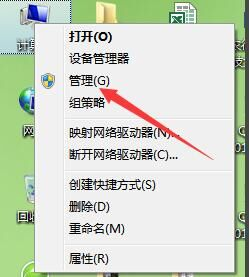
\includegraphics[width=0.2\textwidth]{tu21.jpeg}
\caption{\small 磁盘管理}
\label{tu21}
\end{figure} 

\item 找一个你电脑上比较大的磁盘就可以啦。方法:对着要压缩的分区右击选择“压缩卷即可”,我分了100G,也可以不用这么大,但记得千万别格式化,也别分配盘符,压缩完就可以了。

\item 开始安装与上面一样,就是在安装类型时选择“其他选项”,点击“继续”。

\item 找到其中标有“空闲”的盘符,这个盘符就是我们用于安装Ubuntu的100G空间,别去碰别的盘符,小心弄得到时候Win7不能用了,甚至品牌机自带的隐藏分区也会被破坏。图\ref{tu23}所示
\begin{figure}[!htb] %插图
\centering
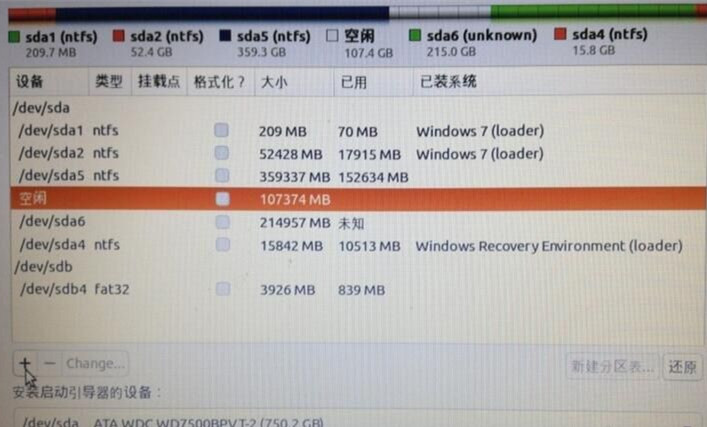
\includegraphics[width=0.4\textwidth]{tu23.jpeg}
\caption{\small 分盘}
\label{tu23}
\end{figure} 

\item 点击左下方的“+”,挂载点:$\slash$,大小:22000MB ,新分区的类型:主分区,新分区的位置:空间起始位置,用于:EXT4日志文件系统;继续“+”,挂载点:$\slash$boot,大小:200MB(一般分100-200MB,但是你的硬盘够大,分1-2G比较好使),新分区的类型:逻辑分区,新分区的位置:空间起始位置,用于:EXT4日志文件系统;挂载点:$\slash$home,大小50G:新分区的类型:逻辑分区,新分区的位置:空间起始位置,用于:EXT4日志文件系统;$\slash$opt、$\slash$swap分区与上面相似,这里就不说了。图\ref{tu24}所示
\begin{figure}[!htb] %插图
\centering
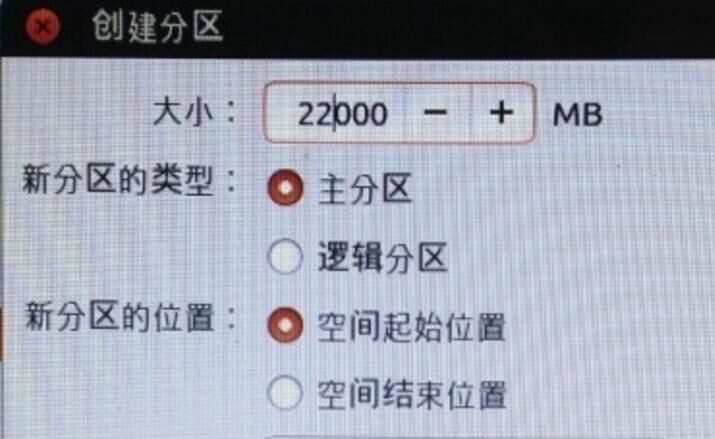
\includegraphics[width=0.3\textwidth]{tu24.jpeg}
\caption{\small /的分区}
\label{tu24}
\end{figure} 
\begin{figure}[!htb] %插图
\centering
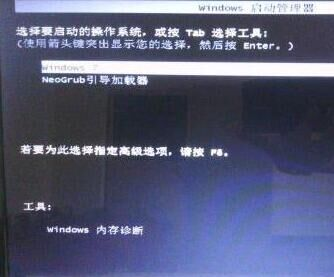
\includegraphics[width=0.3\textwidth]{tu25.jpeg}
\caption{\small 双系统安装开机画面}
\label{tu25}
\end{figure} 

\item 下面步骤与单系统安装一样,就是安装完之后开机界面是这样的\ref{tu25},到目前为止,Ubuntu就安装好了,你可以正常使用了!
\end{enumerate}
\section{Ubuntu的简介}
\subsection{简说Ubuntu}
Ubuntu是基于Linux的免费开源桌面PC操作系统,简单的说,Ubuntu是Linux的一个延伸产品。Ubuntu的开发目的是为了使个人电脑变得简单易用,同时也提供针对企业应用的服务器版本。它主要使用自由、开源的软件。
\subsection{Ubuntu VS Windows}
\begin{enumerate}
\item Linux硬件支持通常比最新的版本的Windows表现更好。

\item Ubuntu 默认采用了类似 Mac 的上下双栏桌面结构,这种方法相对于Windows的单一任务栏,操作效率有着明显的提高。而且Ubuntu菜单中的程序是自动分类的,不需要再像Windows那样在程序菜单中数十个上百个程序中寻找了!

\item Ubuntu不需要磁盘整理。

\item Ubuntu的内存管理和进程调度都很好,而且它有高度可定制性、稳定性。

\item Windows的默认权限是Administrator,平时的操作都在这样的权限下进行。Ubuntu的Administrator为root,而我们平时几乎不需要root,Ubuntu甚至默认不允许使用root登入。我们的大部分程序都运行在低权限上,所能操作的文件只有自己的工作文件夹和几个特殊的文件夹,没有密码谁都改不了重要的东西。所以相比,Ubuntu更安全一点。
\end{enumerate}
\section{Ubuntu的简单使用}
 安装好Ubuntu,接下来就是使用了
\subsection{Ubuntu升级}
  刚按上Ubuntu,需要更新一下,否则许多软件包无法正常使用。
\begin{enumerate}
\item 打开终端:Ctrl+Alt+T 。为了下次方便,打开之后可以在左侧的终端符号除右击选择“锁定到启动器”。如图\ref{tu32}所示

\begin{figure}[!htb] %插图
\centering
\includegraphics[width=0.3\textwidth]{tu32.jpeg}
\caption{\small 终端锁定}
\label{tu32}
\end{figure} 

 \item 在终端输入: sudo apt-get update

~~~~~~~~~~~~~~~~~~~~~~~sudo apt-get upgrade\\
{\color{red}注意:}Uubuntu下使用{\color{red}“sudo”}是以管理员权限运行命令的!
\end{enumerate}
\subsection{Ubuntu常用命令}
\subsubsection{显示文件}
 (1) ls -al

ls是“list”的意思,它主要是显示文件的文件名与相关属性。“-al”表示列出所有的文件详细的权限与属性(包含第一字符为“.”的隐藏文件)。我以我的电脑为例,在终端输入以上命令,可以出现如图\ref{tu31}
\begin{figure}[!htb] %插图
\centering

\includegraphics[width=0.4\textwidth]{tu31.jpeg}
\caption{\small ls -al命令显示}
\label{tu31}
\end{figure} 
\begin{itemize}

\item 第一列代表这个文件的类型与权限

第一个字符是d代表是目录

第一个字符是-代表是文件

第一个字符是l代表是链接文件
\item[*] 接下来3个字符为一组,一共三组。每一组的r是可读,w是可写,x是可执行。这三个权限位置循序是不变的,如果没有权限,就用“-”。这三组权限分别代表:

第一组,文件所有者的权限

第二组,同用户组的权限

第三组,其他非本用户组的权限

\item  第二列代表有多少文件名连接到此节点

\item  第三列代表这个文件的所有者账号

\item  第四列代表这个文件的所属用户组

\item  第五列代表这个文件的容量的大小,默认单位为B

\item  第六列代表这个文件的创建文件日期或者最近的修改时间

\item  第七列代表该文件名
这七个字段的意义重要。尤其第一个字段的9个权限是linux的重点。

\end{itemize}

(2) ls -a

可以显示隐藏文件(.),提前透露在github的秘钥设置时可能会用上。

(3)ls -d */

这条命令可以只显示出目录
\begin{itemize}
\item 我只是列出ls的部分功能,对于更详细的ls用法,可以用“info ls”查看其基础用法。
\end{itemize}
%第一列代表这个文件的类型与权限
 %第一个字符是d代表是目录
% 第一个字符是-代表是文件
% 第一个字符是l代表是链接文件
% 接下来3个字符为一组,一共三组。每一组的r是可读,w是可写,x是可执行。这三个权限位置循序是不变的,如果没有权限,就用“-”。这三组权限分别代表:
 %第一组,文件所有者的权限
% 第二组,同用户组的权限
 %第三组,其他非本用户组的权限
%第二列代表有多少文件名连接到此节点
%第三列代表这个文件的所有者账号
%第四列代表这个文件的所属用户组
%第五列代表这个文件的容量的大小,默认单位为B
%第六列代表这个文件的创建文件日期或者最近的修改时间
%第七列代表该文件名
%这七个字段的意义重要。尤其第一个字段的9个权限是linux的重点
\subsubsection{切换目录}
“cd ..” ~~~~回到上一层目录。

“cd $\backslash$”  ~~~~回到根目录。

“cd ~”  ~~~~回到自己的主文件下即你自己用户名下。

“cd -”  ~~~~回到上一步目录下。

“cd”    ~~~~回到自己的主文件下。

“cd /home/用户名/想要去的目录/想要去的文件或者子目录”  ~~~~~可以从根目录跳转到你想要去的目录或者文件下。

你在执行这些命令时,可以用“ls”查看一下执行这一步后都有哪些目录或文件,很容易就理解了。
\subsubsection{显示目前所在目录}

“pwd”显示目前所在的目录,当前的一个路径


\subsubsection{查看文件的类型}
“file 文件路径”代表可以查看文件的类型。有时候我们对于一个文件的类型不清楚,我们就可以用上面的命令简单的判断一下这个文件的类型了。
\subsubsection{添加打印号打印}
“nl 文件的路径”代表添加行号打印。
\subsubsection{查看非纯文本文件内容} 
“od -t 文件路径”代表可以查看非纯文本文件的内容
\subsubsection{复制、删除、移动}
\begin{enumerate}
\item cp 复制

“cp 源文件 目标文件的路径”  ~~~~把一个文件复制到另一个文件夹下。

如把test文件夹下的11. 移到桌面上,并重命名为22,“cp test$\slash$11.jpg 桌面/22”,用“cd”进入桌面,用“ls”就可以看到桌面出现了一个名为22的图片。上面是在都在家目录下的,如果从用户文件下移到usr里面,用命令“cp test$\slash$11.jpg $\slash$home$\slash$user$\slash$22 ”即可。如图\ref{tu33}
\begin{figure}[!htb] %插图
\centering
\includegraphics[width=0.4\textwidth]{tu33.jpeg}
\caption{\small cp命令显示}
\label{tu33}
\end{figure} 

 如果你想要复制整个文件夹或者目录,需要执行的命令是:“cp -r 源文件夹 目标文件的路径”,此时文件属性会发生变化。所以最好用“cp -a 源文件夹 目标文件的路径”,它留原文件属性,复制完的目录和原目录完全一样。

\item rm 删除

“rm 文件名”代表移除文件。

想要删除一个目录时用“rm -r 目录名”。

{\color{blue}上面所说的“rm -r”一定要先确认以下你是否该目录真的不要了,删除救不不可恢复了,避免误删}。

\item mv 移动

“mv 源文件 目标目录路径”代表移动文件与目录;

“mv 文件名/目录 新的文件名/目录”代表将文件名或者目录名字修改。
\end{enumerate}
\subsubsection{查看文件文件内容且在终端显示}
\begin{enumerate}
\item cat

“cat 文件的路径”代表可以查看这个文件的内容。

\item tac

“tac 文件的路径”代表反向列示文件的内容。与“cat”相比“tac”从最后一行开始在屏幕上显示。
\end{enumerate}
\subsubsection{新建或删除目录}
\begin{enumerate}
\item mkdir

“mkdir 新的目录名”  ~~~~~建立新目录。

新建目录是一层层依次建的,即用cd命令依次进入目录里面创建。不过,也可以在进入你想要建总的目录下用“mkdir -p 目录1/目录2/目录3 ”,可以建立三个依次三个子目录。

\item rmdir

“rmdir 目录名”  ~~~~删除空的目录。

也是cd,进入目录,使用“rmdir”就可以删除刚刚新建的目录,你可以一层层进入删除,可以以用“rkdir -p 目录1/目录2/目录3”,一次性删除。
{\color{red}注意:}“{\color{red}rmdir}”只能删除{\color{red}空的目录},即该目录下没有其他目录和文件,如果你想把所有目录下的东西都删掉,可以是用命令“rm -r 目录名”,此目录下的所有东西都可删掉。
\end{enumerate}
\subsubsection{文件名查找}
\begin{enumerate}
\item whereis

“whereis 文件或目录名”  ~~~~~查找特定文件

whereis查找时间短且可以添加参数找相关的数据

\item locate

“locate 部分文件名” ~~~~~~可以查询出带有这个文件名的文件都会显示出来,在你忘记某个文件的完整文件名时,locate方便好用。但是它不会去硬盘当中访问数据,此时可以用find命令。
\item find
\end{enumerate}
\begin{itemize}
\item  “find 路径 option action” 
\end {itemize}
 ~~~~(1)时间参数:根据更改时间找文件

~~ -mtime n:查找n天前的“一天之内”更改过的文件

~~ -mtime +n:查找n天前更改过的文件

~~ -mtime -n:查找n天之内(含n天之内)更改过的文件

~~ -newer file:file是已经存在的文件,列出比file还要新的文件名

例如:find $\slash$etc -mtime 3~~~~查找$\slash$etc下面3天前的24小时之内更改过的文件

(2)用户或用户组名参数

~~ -uid n:n是用户的账号ID

~~ -gid n:n用户组的账号ID

~~ -use name:name是用户的名称

~~ -group name:name是用户组的名称

~~ -nouser:寻找文件的所有者不存在$\slash$etc$\slash$passwd中的文件

~~ -nogroup:寻找文件的所有者组不存在于$\slash$etc$\slash$group中的文件

例如:find $\slash$home -user tanlin ~~~~可以查出tanlin这个用户的所有文件

(3)文件权限及名称参数

~~ -name filename:查找文件名为filename的文件

~~ -size +/-规格:查找比规格大的或小的文件;规格有:c ~~~~byte,k~~~~~1024byte

~~ -type 类型:查找某种类型的文件;f~~~~一般正规文件,b/c~~~~设备文件,d~~~~目录,l~~~~~~链

~~ 接文件,s~~~~socket,p~~~~FIFO

~~ -perm mode:mode是类似chomd的属性值,是个数,查找文件权限“刚好等于”mode~~的文件

~~ -perm +mode:查找文件权限“包含任一mode的权限”的文件

~~ -perm -mode:查找文件权限“全部包含mode权限”的文件

例如:find $\slash$var -type s  ~~~~找持股/var目录下文件类型为socket的文件名有哪些

(4)其他可进行操作

~~ -exec 命令:根据命令查找的文件

~~ -print:将结果打印到屏幕上,这是默认操作

从上面介绍find指令的用法可以看出,find是很强大的查找命令,也是我们经常用的。
\subsubsection{计算某个程序/指令的耗时}
“time <command> [<arguments...>]” ~~~~我们经常用来计算某个程序或者指令的运行耗时(real),用户态cpu耗时(user),系统态cpu耗时(sys)

如图\ref{tu35}所示,描述的是codeblocks这个程序的耗时。
\begin{figure}[!htb] %插图
\centering
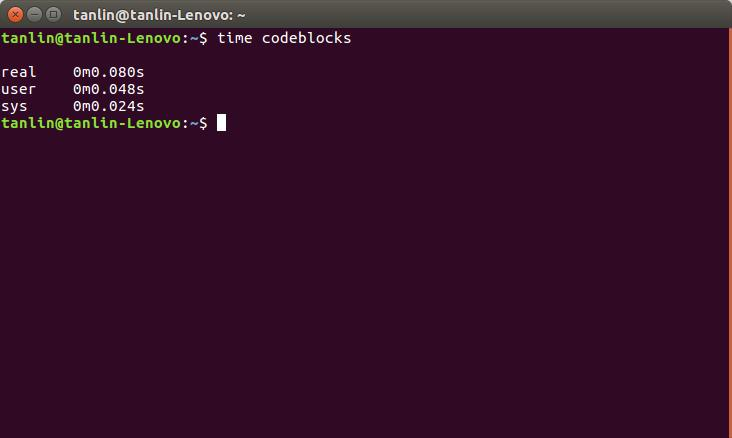
\includegraphics[width=0.4\textwidth]{tu35.jpeg}
\caption{\small time命令显示}
\label{tu35}
\end{figure} 
\subsubsection{vim程序编辑器}
vim分为三种模式,一般模式、编辑模式、命令行模式,我们一般常用前两种

(1)vim进入一般模式

vim 新文件名或者已有的文件名  (要在文件的目录下执行这步,用vim也可以新建一个文档,但要表明它的类型)

(2)vim进入编辑模式

在一般模式下按“A,a,I,i,O,o,R,r”都可进入编辑模式了,你就可以编写你需要的内容

“Esc” 退出进入一般模式

如果你想退出编辑,先按“Esc”再按“:wq”,就可以保存退回到终端
\subsubsection{两个连续明令豫剧合并成一句}
“|”相当与一个管道,用于传输文件,“grep”相当与过滤。

“命令A|grep 命令B”可用于两个语句可以合并成一个语句,即,A的输出作为B的输入。

\subsubsection{挂载镜像文件}
\begin{lstlisting}
sudo mount -o loop /文件路径 /mnt
\end{lstlisting}
\subsubsection{安装文件}
\begin{lstlisting}
sudo apt-get install 软件名(此时软件名是软件源中有的)
\end{lstlisting}
\subsubsection{sudo常用命令}
\begin{lstlisting}
1、sudo apt-get

查看一下apt-get的常用命令
\end{lstlisting}
如图\ref{tu34}
\begin{figure}[!htb] %插图
\centering
\includegraphics[width=0.4\textwidth]{tu34.jpeg}
\caption{\small apt-get命令显示}
\label{tu34}
\end{figure} 
\begin{lstlisting}
2、sudo apt-cache search +文件名

可以查看这个软件是否在软件源里
\end{lstlisting}
\begin{lstlisting}
3、apt-cache depends 软件名

查询软件可以依赖哪些包
\end{lstlisting}
\begin{lstlisting}
4、sudo apt-get autoclean

 清理旧版本的软件缓存
\end{lstlisting}
\begin{lstlisting}
5、sudo apt-get clean

清理所有软件缓存
\end{lstlisting}
\begin{lstlisting}
6、sudo apt autoremove +文件名

卸载某些文件夹或者文档
\end{lstlisting}
\begin{lstlisting}
7、gnome-system-monitor

关闭一些正在运行的进程,一般用在一个软件卡了的时候。也可以用“killall+程序名”。
\end{lstlisting}
在这里我只是说了一些常用的Ubuntu命令,Ubuntu的命令很多你可以参照网址\url{http://www.jb51.net/os/Ubuntu/56362.html}或者参考书{\color{red}《鸟哥的linux私房菜》}。
\subsection{Ubuntu常用快捷键}
1、Ctrl+Shift+T 打开终端

2、以下在终端中用

  (1)Ctrl+c~~~~中断终端进程

  (2)Ctrl+l~~~~清屏

 (3)Ctrl+a~~~~跳到行首

 (4)Ctrl+d~~~~从光标向右删除

 (5)Tab~~~~~~~输入首字补全文件名,节省时间

  (6)Ctrl+d~~~~在没有输入指令时表示关闭终端

3、Ctrl+f~~~~~~在文档中查询文档关键词 
 
4、Ctrl+h~~~~~~查看隐藏文件

5、Alt+	Tab~~~切换窗口

6、可以在桌面的左上角的搜索窗口,在上面输上你想要的文件或者程序名,就可以被找到。

Ubuntu的一些常用快捷键,我暂时只列这些,你可以参考网上的Linux的快捷键大全。
\section{结束语}
自本人使用Ubuntu以来,觉得其真心不错,这里只是说了一个Ubuntu的安装教程和命令的简单应用,适合Linux初学者使用,希望可以帮助大家了解并喜欢上Ubuntu,祝大家使用愉快!

\end{document}
